%%%%%%%%%%%%%%%%%%%%%%%%%%%%%%%%%%%%%%%%%%%%%%%%%%%%%%%%%%%%%%%%%%%%%%%%%%%%%%%%%%%%%%%%%%%%%%%%%%%
\documentclass[11pt]{beamer}
\usetheme[block=fill]{metropolis}
\usepackage[utf8]{inputenc}
\usepackage[spanish]{babel}
\usepackage{amsmath}
\usepackage{amsfonts}
\usepackage{amssymb}
\usepackage{graphicx}

% numeros con punto decimal, no coma
\decimalpoint

% para la bibliografia
\usepackage[style=verbose,backend=bibtex]{biblatex}
\bibstyle{abbrv}

% codigo de R
\usepackage{listings}
\usepackage{color}

% para las tablitas
\usepackage{booktabs}

% para tablas de colores
\usepackage{xcolor,colortbl}
\usepackage{multirow}

%\usefonttheme[onlymath]{mathserif}
%\usepackage{mathpazo} 
\usepackage{eulervm}                 %
\usepackage[scaled ]{helvet}  

% intento de incluir animaciones
\usepackage{movie15}

%%%%%%%%%%%%%%%%%%%%%%%%%%%%%%%%%%%%%%%%%%%%%%%%%%%%%%%%%%%%%%%%%%%%%%%%%%%%%%%%%%%%%%%%%%%%%%%%%%%

% retoques graficos para el codigo en R
\newsavebox{\caja}

%%%%%%%%%%%%%%%%%%%%%%%%%%%%%%%%%%%%%%%%%%%%%%%%%%%%%%%%%%%%%%%%%%%%%%%%%%%%%%%%%%%%%%%%%%%%%%%%%%%

% comandos para tablas
\newcommand{\bordes}[1]{\renewcommand{\arraystretch}{#1}}
\definecolor{gray}{rgb}{0.5,0.5,0.5}
\definecolor{gris}{gray}{0.925}
\definecolor{gris2}{gray}{0.8}

%%%%%%%%%%%%%%%%%%%%%%%%%%%%%%%%%%%%%%%%%%%%%%%%%%%%%%%%%%%%%%%%%%%%%%%%%%%%%%%%%%%%%%%%%%%%%%%%%%%

% bibliografia
\addbibresource{referencias_estacionariedad.bib}
\addbibresource{referencias_fisiologia.bib}
\addbibresource{referencias_otros.bib}
\addbibresource{referencias_mixto.bib}

\renewcommand{\footnotesize}{\tiny}

%%%%%%%%%%%%%%%%%%%%%%%%%%%%%%%%%%%%%%%%%%%%%%%%%%%%%%%%%%%%%%%%%%%%%%%%%%%%%%%%%%%%%%%%%%%%%%%%%%%

% abreviaciones varias
\newtheorem{defn}{Definici\'on}
\newtheorem{thrm}{Teorema}
\newtheorem{demostracion}{Demostraci\'on}
\newtheorem{prop}{Proposici\'on}

\newcommand{\R}{\mathbb{R}}
\newcommand{\intR}{\int_{-\infty}^{\infty}}
\newcommand{\intZ}{\int_{-\infty}^{0}}
\newcommand{\intPI}{\int_{-\pi}^{\pi}}
\newcommand{\simint}[1]{\int_{- #1 }^{ #1 }}
\newcommand{\prima}{^{\prime}}

\newcommand{\ddd}{$\delta$}
\newcommand{\dirac}{$\delta$  de Dirac}

\newcommand{\aste}[1]{\widehat{ #1 }^{\star}}
\newcommand{\est}[1]{\widehat{ #1 }}

\newcommand{\COS}[1]{\mathrm{cos}\left( #1 \right)}
\newcommand{\SEN}[1]{\mathrm{sen}\left( #1 \right)}

\newcommand{\E}[1]{\mathrm{E}\left[ #1 \right]}
\newcommand{\Var}[1]{\mathrm{Var}\left( #1 \right)}
\newcommand{\Cov}[1]{\mathrm{Cov}\left( #1 \right)}
\newcommand{\abso}[1]{\left| #1 \right|}

%%%%%%%%%%%%%%%%%%%%%%%%%%%%%%%%%%%%%%%%%%%%%%%%%%%%%%%%%%%%%%%%%%%%%%%%%%%%%%%%%%%%%%%%%%%%%%%%%%%

% titulo y fecha
\author{Julio Cesar Enciso Alva}
\title{Estacionariedad d\'ebil}
\subtitle{Detecci\'on en series electrofisiol\'ogicas}
%\setbeamercovered{transparent} 
\setbeamertemplate{navigation symbols}{} 
%\logo{} 
\institute{Instituto de Ciencias B\'asicas e Ingenier\'ia\\ 
Universidad Aut\'onoma del Estado de Hidalgo} 
\date{\emph{Neuroscience Short Course}\\
6 de julio de 2017} 
%\subject{} 

%%%%%%%%%%%%%%%%%%%%%%%%%%%%%%%%%%%%%%%%%%%%%%%%%%%%%%%%%%%%%%%%%%%%%%%%%%%%%%%%%%%%%%%%%%%%%%%%%%%

\begin{document}

\begin{frame}
\titlepage
\end{frame}

%\begin{frame}
%\tableofcontents
%\end{frame}

%%%%%%%%%%%%%%%%%%%%%%%%%%%%%%%%%%%%%%%%%%%%%%%%%

%\section{Introducci\'on}

\begin{frame}\frametitle{Motivaci\'on}
El estudio y diagnóstico de una gran cantidad de enfermedades depende de nuestra habilidad para
registrar y analizar se\~nales electrofisiol\'ogicas. \\

%\vspace{3em}
\vspace{2em}

Se suele asumir que estas se\~nales son complejas: no lineales, \alert{no estacionarias} y sin equilibrio 
por naturaleza. Pero usualmente no se comprueban formalmente estas propiedades.
\end{frame}

%%%%%%%%%%%%%%%%%%%%%%%%%%%%%%%%%%%%%%%%%%%%%%%%%

\begin{frame}\frametitle{Motivaci\'on: formalidad}
\begin{figure}[h]
\centering
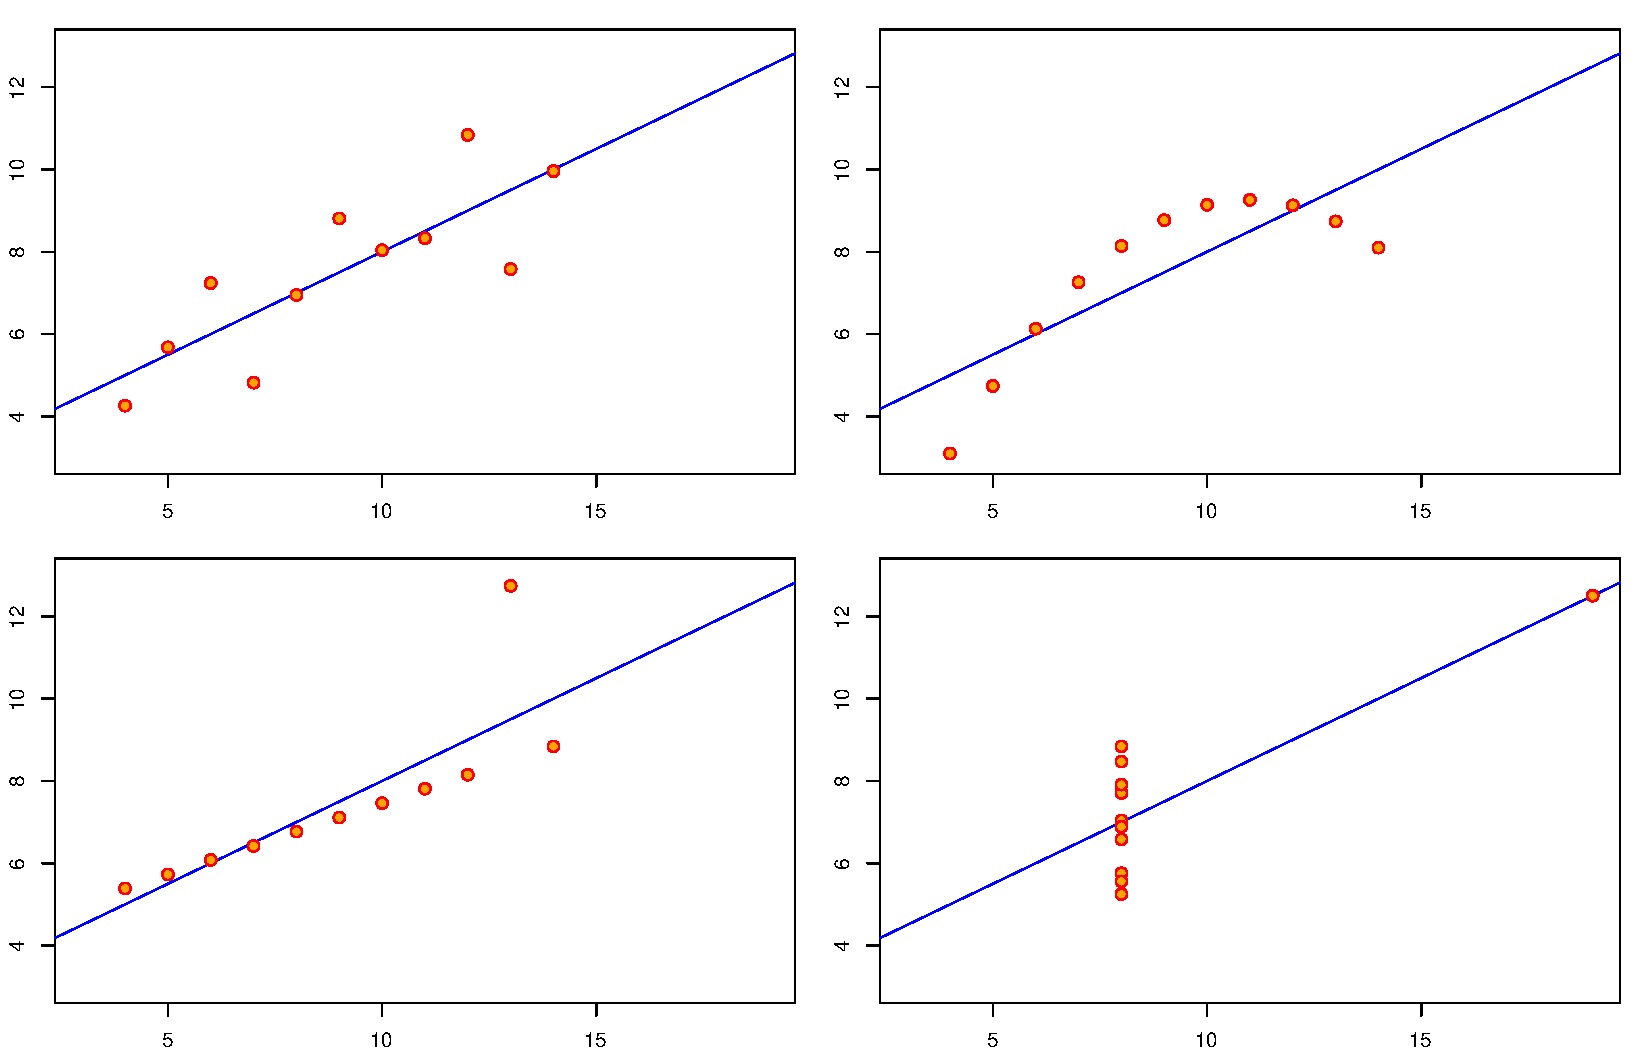
\includegraphics[width=0.85\linewidth]{./img_old/anscombe.pdf} 
\end{figure}
\end{frame}

%%%%%%%%%%%%%%%%%%%%%%%%%%%%%%%%%%%%%%%%%%%%%%%%%

\section{Conceptos}

\begin{frame}\frametitle{Conceptos}
\begin{defn}[Estacionariedad d\'ebil]
Un proceso estoc\'astico es d\'ebilmente estacionario si y s\'olo si para cualesquiera tiempos 
admisibles $t$, $s$ se tiene que
\begin{itemize}
\item $\E{X(t)} = \mu_X$
\item $\Var{X(t)} = \sigma^{2}_X$
\item $\Cov{X(t),X(s)} = \rho_X (s-t)$
\end{itemize}
Con $\mu_X$, $\sigma^{2}_X$ constantes, $\rho_X(\tau)$ \'unicamente depende de $\tau$
\end{defn}
\end{frame}

%%%%%%%%%%%%%%%%%%%%%%%%%%%%%%%%%%%%%%%%%%%%%%%%%

%\begin{frame}\frametitle{Conceptos}
%\begin{defn}[Funci\'on de densidad espectral (SDF)]
%Sea $\{X(t)\}$ un proceso estoc\'astico a tiempo continuo, d\'ebilmente estacionario
%\begin{equation*}
%h(\omega) = \lim_{T\rightarrow \infty} \E{ \frac{ \left| G_T(\omega) \right|^{2}}{2 T} }
%\end{equation*}
%Donde $\displaystyle G_T (\omega) = \frac{1}{\sqrt{2 \pi}} \int_{-T}^{T} X(t) e^{-i \omega t} dt$
%\end{defn}
%\end{frame}

%%%%%%%%%%%%%%%%%%%%%%%%%%%%%%%%%%%%%%%%%%%%%%%%%

\begin{frame}\frametitle{Espectro de potencias vs Autocorrelaci\'on}
\begin{thrm}[Wiener-Khinchin]
Una condici\'on suficiente y necesaria para que $\rho$ sea funci\'on de autocorrelaci\'on para 
alg\'un proceso a tiempo continuo d\'ebilmente estacionario y estoc\'asticamente continuo, 
$\{X(t)\}$,  es que exista una funci\'on $F$ tal que
%\begin{itemize}
%\item Es mon\'otonamente creciente
%\item $F(-\infty) = 0$
%\item $F(+\infty) = 1$
%\item Para todo $\tau \in \R$ se cumple que
\begin{equation*}
\rho(\tau) = \intR e^{i \omega \tau} dF(\omega)
\end{equation*}
%\end{itemize}
\end{thrm}
\end{frame}

%%%%%%%%%%%%%%%%%%%%%%%%%%%%%%%%%%%%%%%%%%%%%%%%%

\begin{frame}\frametitle{Espectro evolutivo}
Se consideran procesos no-estacionarios, estoc\'asticamente continuos, de media cero y varianza 
finita, y que admitan una representaci\'on de la forma
\begin{equation*}
X(t) = \intPI A(t,\omega) e^{i t \omega} dZ(\omega)
\end{equation*}
tal que 
\begin{itemize}
\item $\Cov{dZ(\omega),dZ(\lambda)} = 0 \Leftrightarrow \omega \neq \lambda$
\item $\E{\abso{dZ(\omega)}^{2}} = \mu(\omega)$
\end{itemize}

El \textbf{espectro evolutivo} fue definido por Priestley \footcite{Priestley65} como
\begin{equation*}
f(t,\omega) = \abso{A(t,\omega)}^{2}
\end{equation*}
\end{frame}

%%%%%%%%%%%%%%%%%%%%%%%%%%%%%%%%%%%%%%%%%%%%%%%%%

\begin{frame}\frametitle{La base de la prueba}
Sup\'ongase que puede* expresarse
\begin{equation*}
X_t = \int_{-\pi}^{\pi} A_t(\omega) e^{i\omega t} \, d\xi(\omega)
\end{equation*}

\pause
\begin{center}
$X_t$ es estacionaria $\Rightarrow A_t(\omega)$ es constante $\Rightarrow f_t(\omega)$ es constante
\end{center}

\pause
La contrapositiva
\begin{center}
$f_t(\omega)$ no constante $\Rightarrow X_t$ \textbf{no} es estacionaria
\end{center}

\underline{Por hacer:} Encontrar un \textit{buen} estimador para $f_t$
\end{frame}

%%%%%%%%%%%%%%%%%%%%%%%%%%%%%%%%%%%%%%%%%%%%%%%%%

\section{Metodolog\'ia, teor\'ia}

\begin{frame}\frametitle{Descomposición cl\'asica usando loess}

Filtro no-param\'etrico para generar las series de tiempo
\begin{equation*}
X_t = T_t + S_t + R_t
\end{equation*}\\

Tales que:\\
\begin{description}
\item[$S_t$] Función peri\'odica suave (frecuencia dada)
\\ \textbf{Componente estacional}
\item[$T_t$] Función suave, no necesariamente peri\'odica
\\ \textbf{Tendencia}
\item[$R_t$] Residuo
\end{description}

Comando en R: \textcolor{red}{\texttt{stl()}}
\end{frame}

%%%%%%%%%%%%%%%%%%%%%%%%%%%%%%%%%%%%%%%%%%%%%%%%%

\begin{frame}[fragile]
\begin{figure}[h]
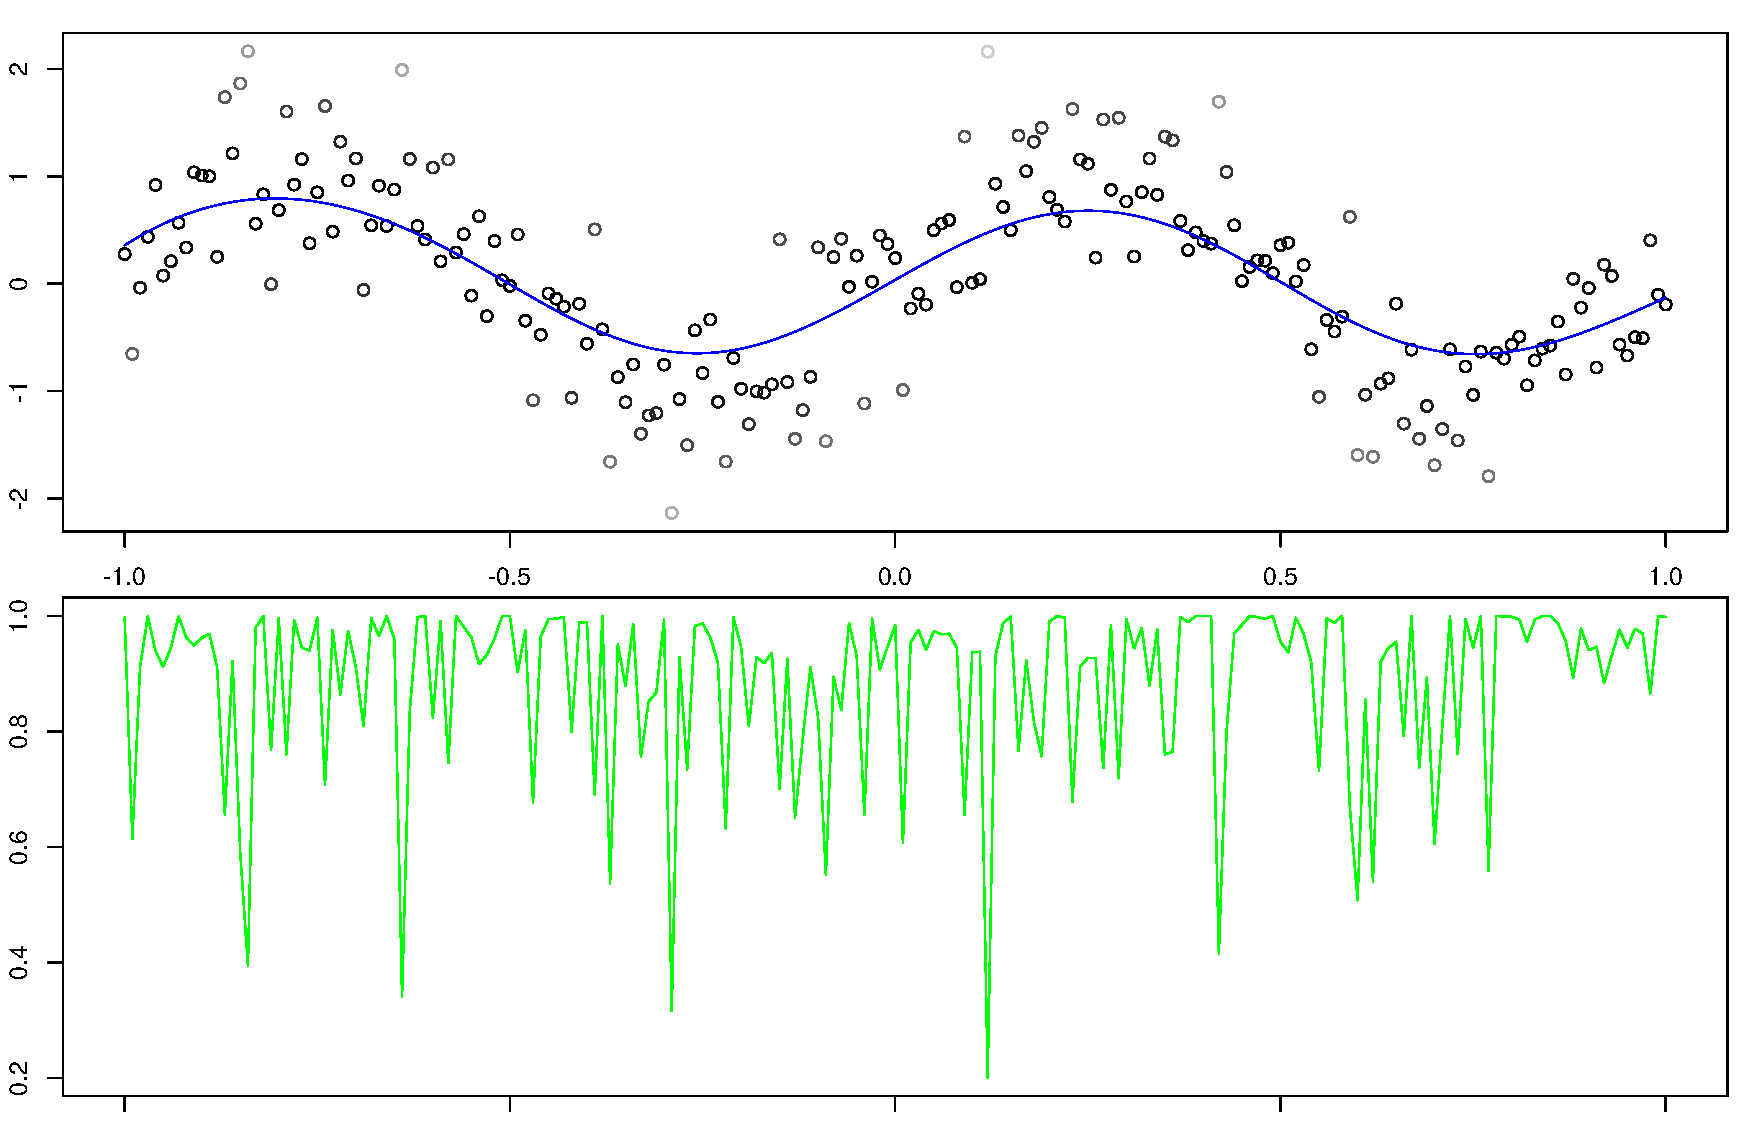
\includegraphics[width=\linewidth]{./img_old/stl_demo2_1.pdf} 
\end{figure}
%\begin{center}
%\includemovie{3em}{3em}{./img_old/stl_demo2_gif.gif}
%\end{center}
\end{frame}

%%%%%%%%%%%%%%%%%%%%%%%%%%%%%%%%%%%%%%%%%%%%%%%%%

\begin{frame}\frametitle{El estimador de doble ventana}
\begin{defn}[Estimador de doble ventana]
Se define a $\est{f}$, estimador para la $f$, como
\begin{equation*}
\widehat{f}(t,\omega) = \int_{t-T}^{t} w_{T'}(u) \lvert U(t-u,\omega) \lvert^{2} du
\end{equation*}

%\begin{itemize}
%\item $U(t,\omega) = \int_{t-T}^{t} g(u) X({t-u}) e^{i \omega (t-u)} du$
%
%\item $2\pi \int_{-\infty}^{\infty} \lvert g(u) \lvert^{2} du = 
%\int_{-\infty}^{\infty} \lvert \Gamma(\omega) \lvert^{2} d\omega = 1$
%\item $w_{\tau}(t) \geq 0$ para cualesquiera $t$, $\tau$
%\item $w_{\tau}(t) \rightarrow 0$ cuando $\lvert t \lvert \rightarrow \infty$, para todo $\tau$
%\item $\int_{-\infty}^{\infty} w_{\tau}(t) dt = 1$ para todo $\tau$
%\item $ \int_{-\infty}^{\infty} \left( w_{\tau}(t) \right)^{2} dt < \infty$ para todo $\tau$
%\item $\exists C$ tal que  
%$ \lim_{\tau\rightarrow\infty} \tau \int_{-\infty}^{t} \abso{ W_{\tau}(\lambda) }^{2} d\lambda = C$
%\end{itemize}
\end{defn}
\end{frame}

%%%%%%%%%%%%%%%%%%%%%%%%%%%%%%%%%%%%%%%%%%%%%%%%%

\begin{frame}%\frametitle{}
\begin{prop}
El estimador de doble ventana $\widehat{f}$ tiene las siguientes propiedades
\begin{itemize}
\item $\displaystyle \E{\est{f}(t,\omega)} \approx f(t,\omega)$
\item $\displaystyle \Var{\est{f}(t,\omega)} \approx 
\frac{C}{\tau} f^{2}(t,\omega) \intR \abso{\Gamma (\theta)}^{4} d\theta$
\item $\displaystyle \Cov{\est{f}(t_1,\omega_1) , \est{f}(t_2,\omega_2)} \approx \intR \intR
w_\tau (u) w_\tau(v) \Cov{ \abso{U(t_1-u,\omega_1)}^{2} , \abso{U(t_2-u,\omega_2)}^{2} } du dv$
\end{itemize}
\end{prop}
\end{frame}

%%%%%%%%%%%%%%%%%%%%%%%%%%%%%%%%%%%%%%%%%%%%%%%%%

\begin{frame}%\frametitle{}
M\'as a\'un, puede escribirse
\begin{equation*}
Y(t,\omega) = \log \left( f(t,\omega) \right) + \varepsilon(t,\omega)
\end{equation*}
donde las variables $\varepsilon(t,\omega)$ satisfacen que
\begin{itemize}
\item $\displaystyle \E{\varepsilon(t,\omega)} = 0$
\item $\displaystyle \Var{\varepsilon(t,\omega)}
\approx \frac{C}{\tau} \intR \abso{\Gamma (\theta)}^{4} d\theta$
\end{itemize}

En particular, se puede usar num\'ericamente el que
\begin{equation*}
\sum_{i = 1 }^{N} \left( Y(t,\omega_i) - \overline{Y}(\bullet,\omega_i) \right)^{2} 
\sim \sigma^{2} \chi^{2}(N)
\end{equation*}
con $\sigma^{2} = \Var{\varepsilon(t,\omega)}$, y
$\overline{Y}(\bullet,\omega) = \frac{1}{M} \sum_{j=1}^{M} Y(t_j,\omega)$.
\end{frame}

%%%%%%%%%%%%%%%%%%%%%%%%%%%%%%%%%%%%%%%%%%%%%%%%%

\section{Metodolog\'ia, pr\'actica}

\begin{frame}\frametitle{Registro de PSG}
\begin{figure}
\centering
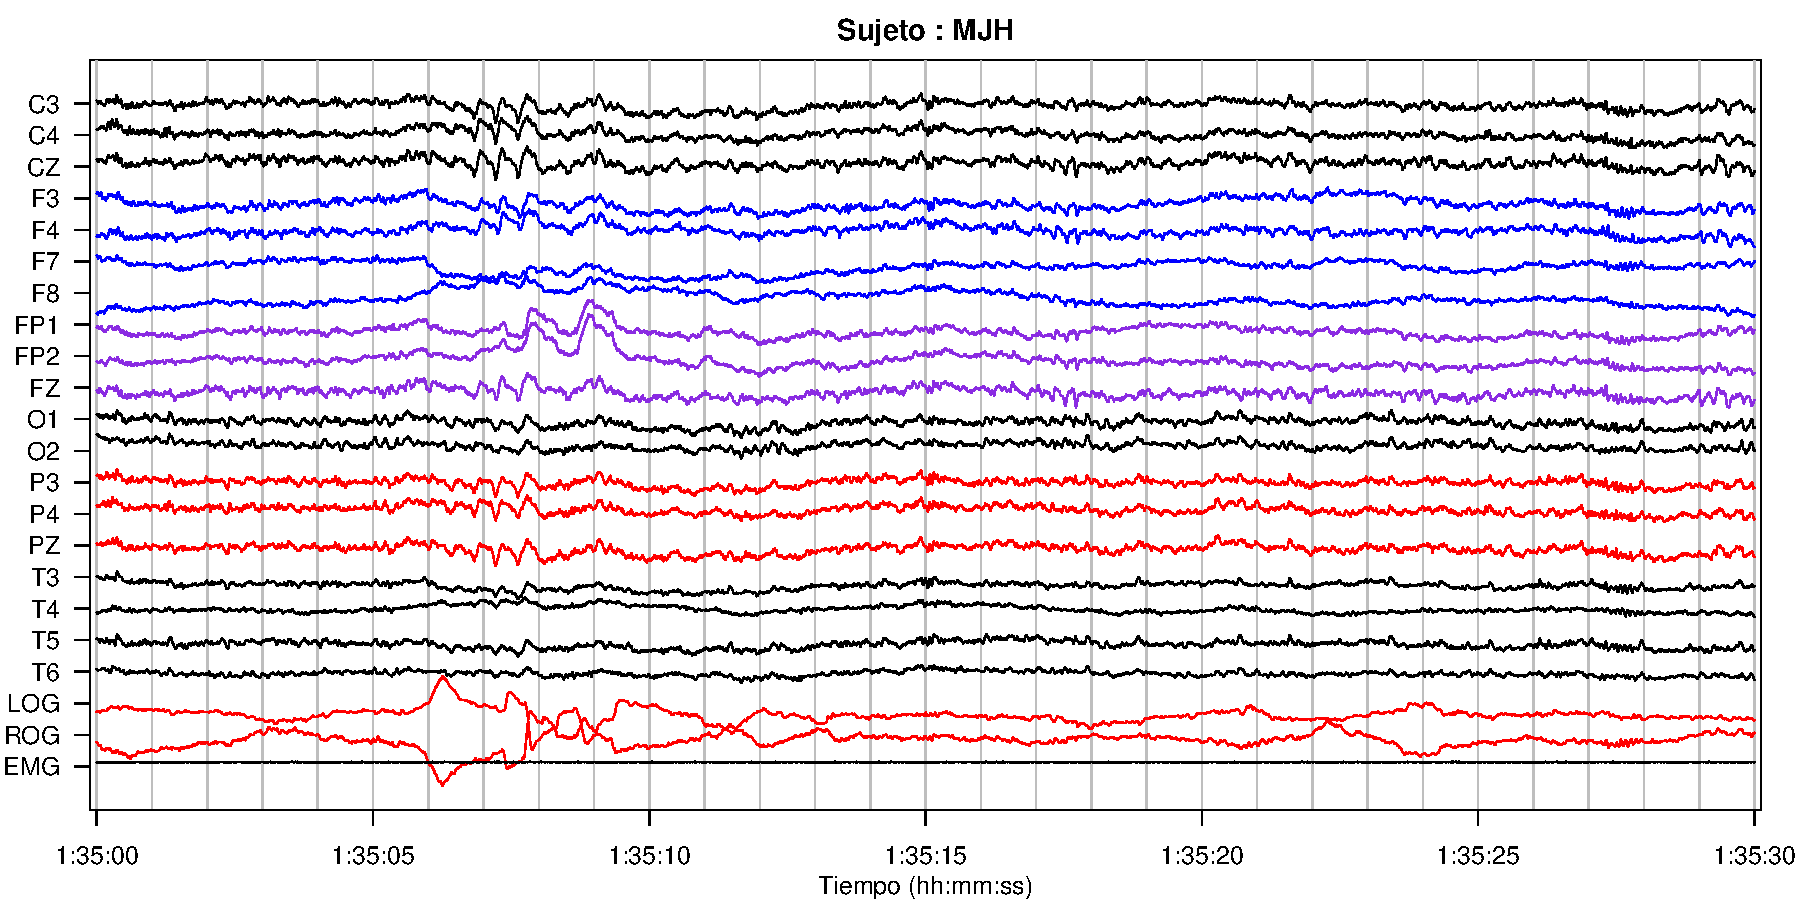
\includegraphics[width=0.9\linewidth]{./img_ejemplos/MJH_190_PDG_lucirse_PSG.pdf}
\caption{PSG: 19 electrodos EEG, 4 electrodos EOG (horizontal y vertical), 2 electrodos EMG en 
m\'usculos submentonianos}
\end{figure}
\end{frame}

%%%%%%%%%%%%%%%%%%%%%%%%%%%%%%%%%%%%%%%%%%%%%%%%%

\begin{frame}[fragile]\frametitle{Espectro estimado}

\begin{center}
\begin{tabular}{cc}
%\includemovie{5em}{5em}{./img_old/priestley_spectra_full.gif}
%\includemovie{5em}{5em}{./img_old/priestley_spectra_small.gif}
pelis
\end{tabular} 
\end{center}

%Por hacer: reescribir las ecuaciones del paper priestley68
\end{frame}

%%%%%%%%%%%%%%%%%%%%%%%%%%%%%%%%%%%%%%%%%%%%%%%%%

\begin{frame}[fragile]
\begin{tabular}{cc}
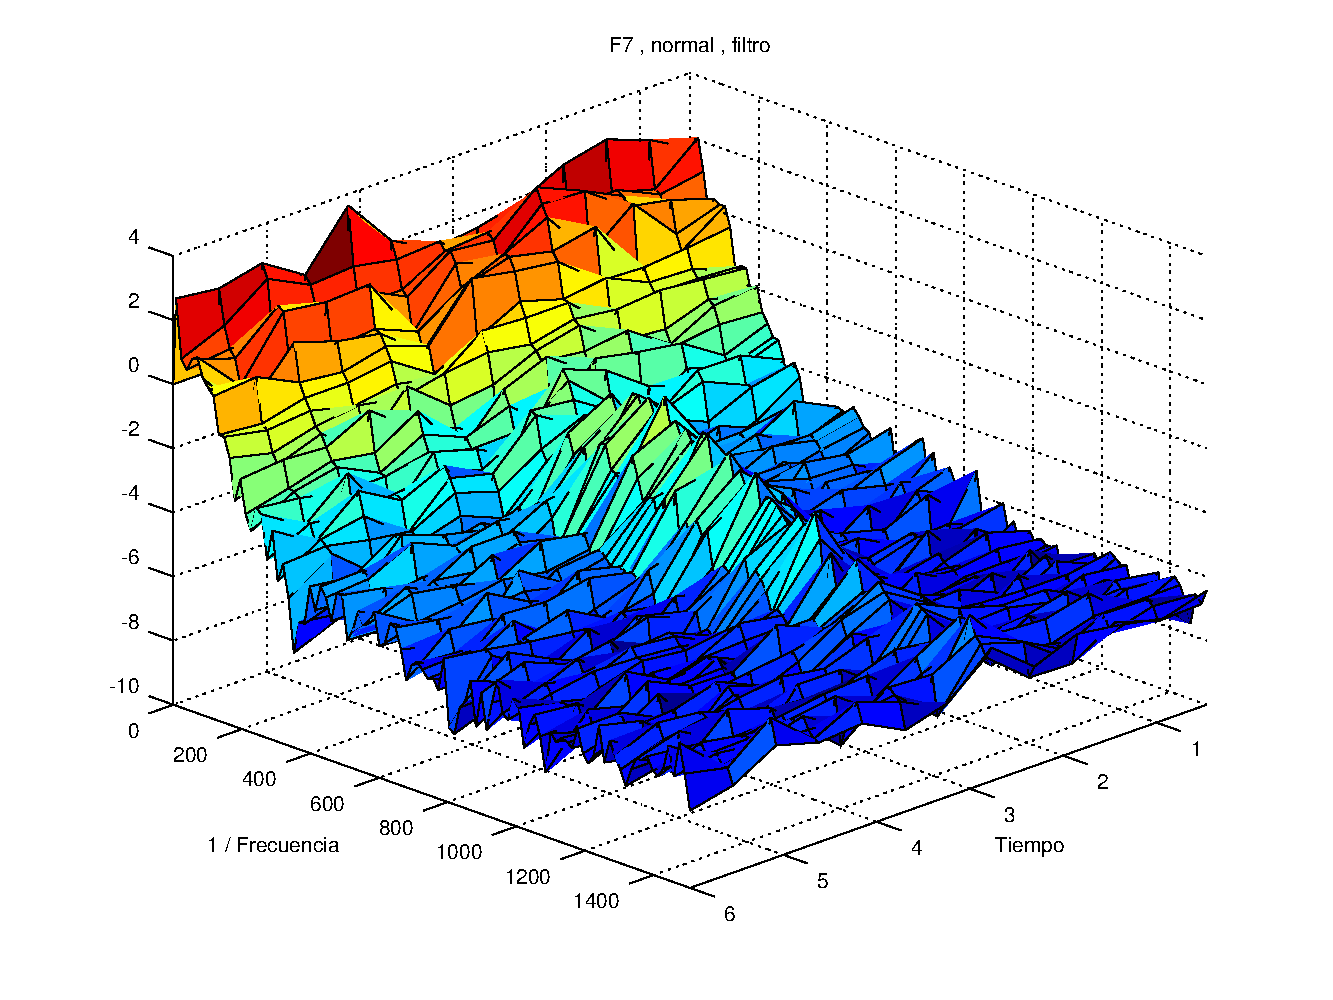
\includegraphics[width=0.5\linewidth]{./img_old/n7f.pdf} 
&
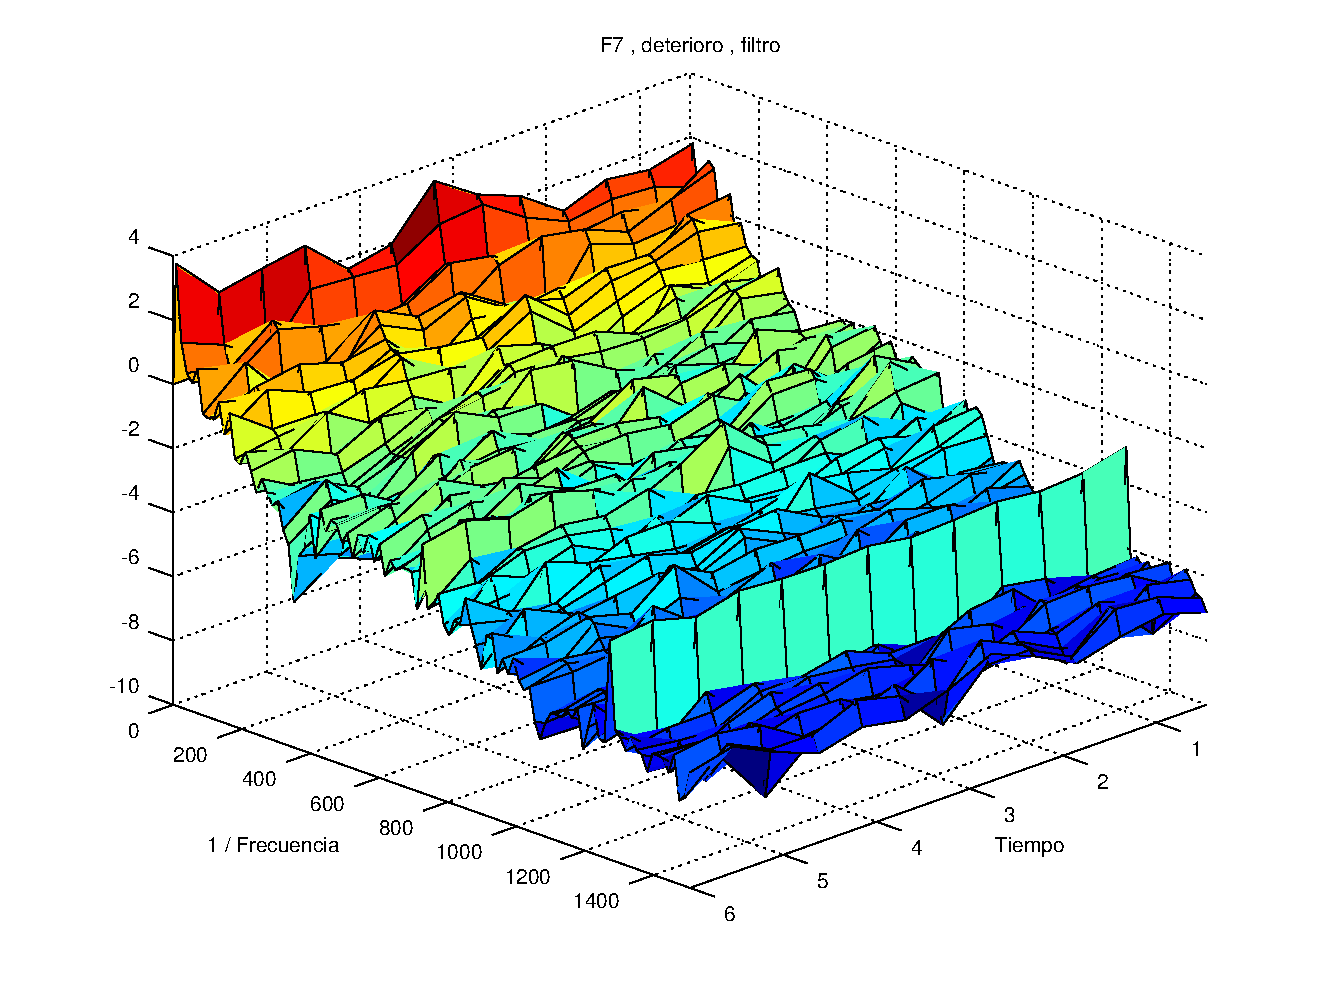
\includegraphics[width=0.5\linewidth]{./img_old/d7f.pdf} 
\\
\begin{lstlisting}
T      : 0 
I+R    : 0 
T+I+R  : 0 
\end{lstlisting}
&
\begin{lstlisting}
T      : 4.36434e-07 
I+R    : 0.0001575723 
T+I+R  : 6.98897e-06 
\end{lstlisting}
\end{tabular}
\end{frame}

%%%%%%%%%%%%%%%%%%%%%%%%%%%%%%%%%%%%%%%%%%%%%%%%%

\begin{lrbox}{\caja}%
\begin{lstlisting}[caption={}]
Priestley-Subba Rao stationarity Test for datos
-----------------------------------------------
Samples used              : 3072 
Samples available         : 3069 
Sampling interval         : 1 
SDF estimator             : Multitaper 
  Number of (sine) tapers : 5 
  Centered                : TRUE 
  Recentered              : FALSE 
Number of blocks          : 11 
Block size                : 279 
Number of blocks          : 11 
p-value for T             : 0.4130131 
p-value for I+R           : 0.1787949 
p-value for T+I+R         : 0.1801353 
\end{lstlisting}
\end{lrbox}%

\begin{frame}[fragile]\frametitle{Resultado esperado}
\begin{figure}
\scalebox{0.7}{\usebox{\caja}}
%\caption{La prueba de Priestley-Subba Rao se encuentra implementada en R como la funci\'on 
%\texttt{stationarity()}, del paquete \texttt{fractal}}
\end{figure}
\end{frame}

%%%%%%%%%%%%%%%%%%%%%%%%%%%%%%%%%%%%%%%%%%%%%%%%%

\begin{frame}\frametitle{Patrones visuales}
\begin{figure}
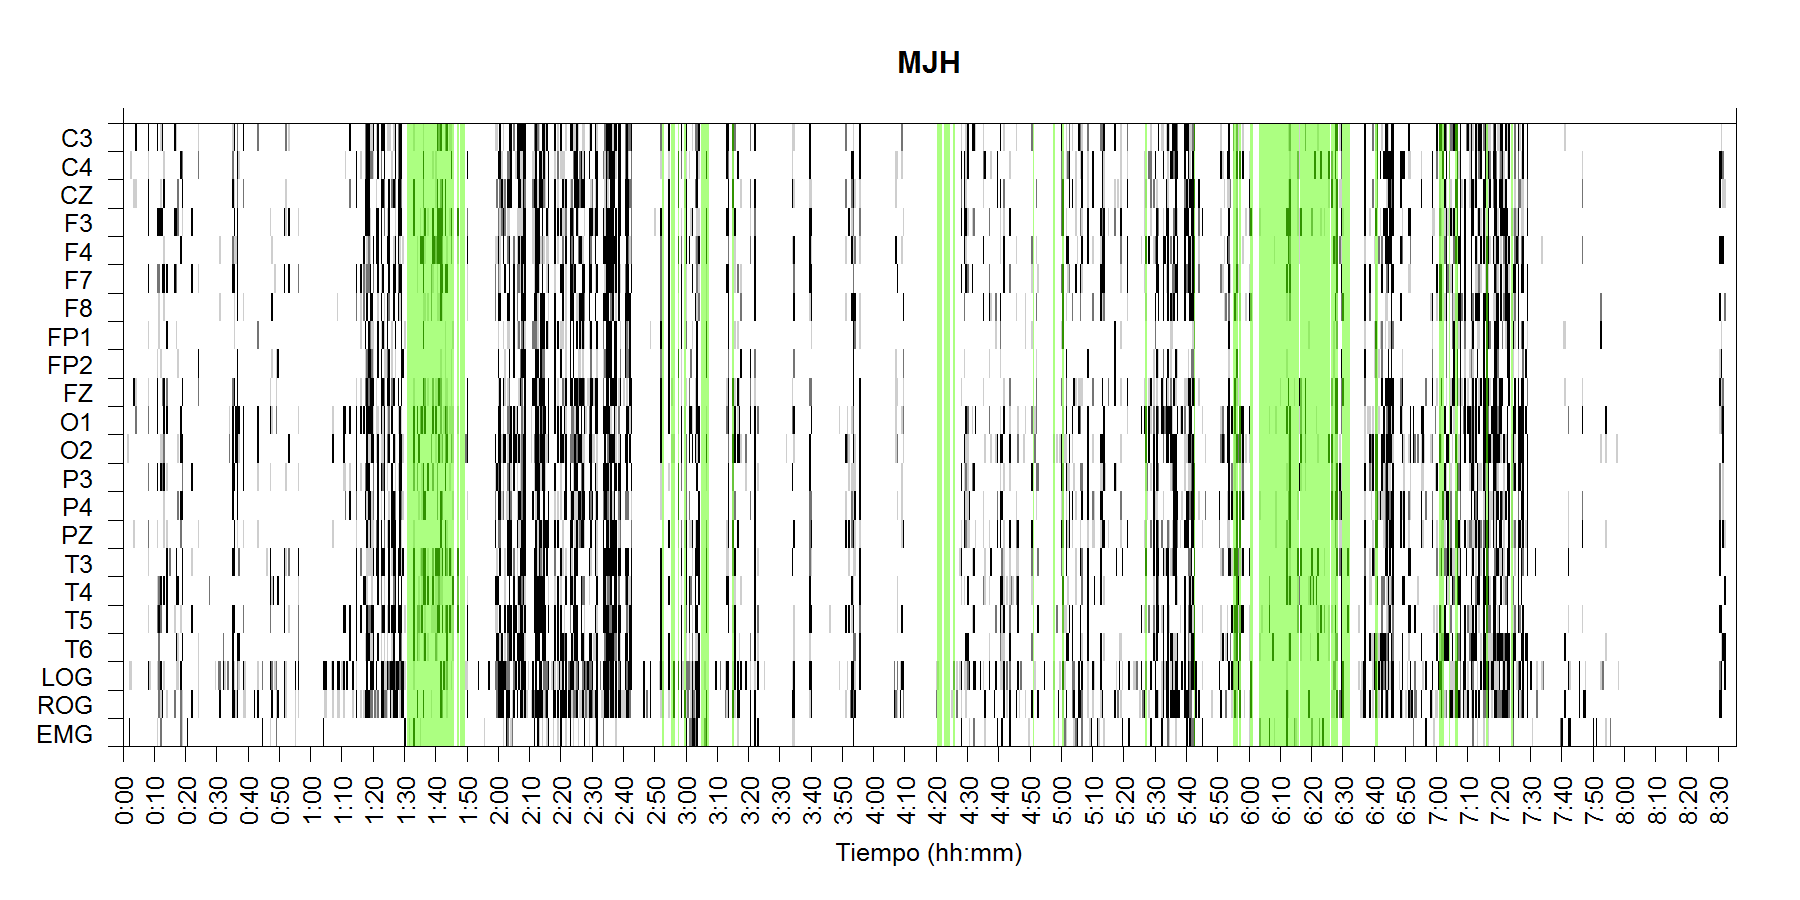
\includegraphics[width=\textwidth]
{./img_ejemplos/MJNNVIGILOS_est.png}
\caption{Disposici\'on gr\'afica para los resultados de la prueba PSR. En verde el sue\~no MOR.}
\end{figure}
\end{frame}

%%%%%%%%%%%%%%%%%%%%%%%%%%%%%%%%%%%%%%%%%%%%%%%%%

\begin{frame}\frametitle{Efecto del tama\~no de la \'epoca}
\begin{figure}
\centering
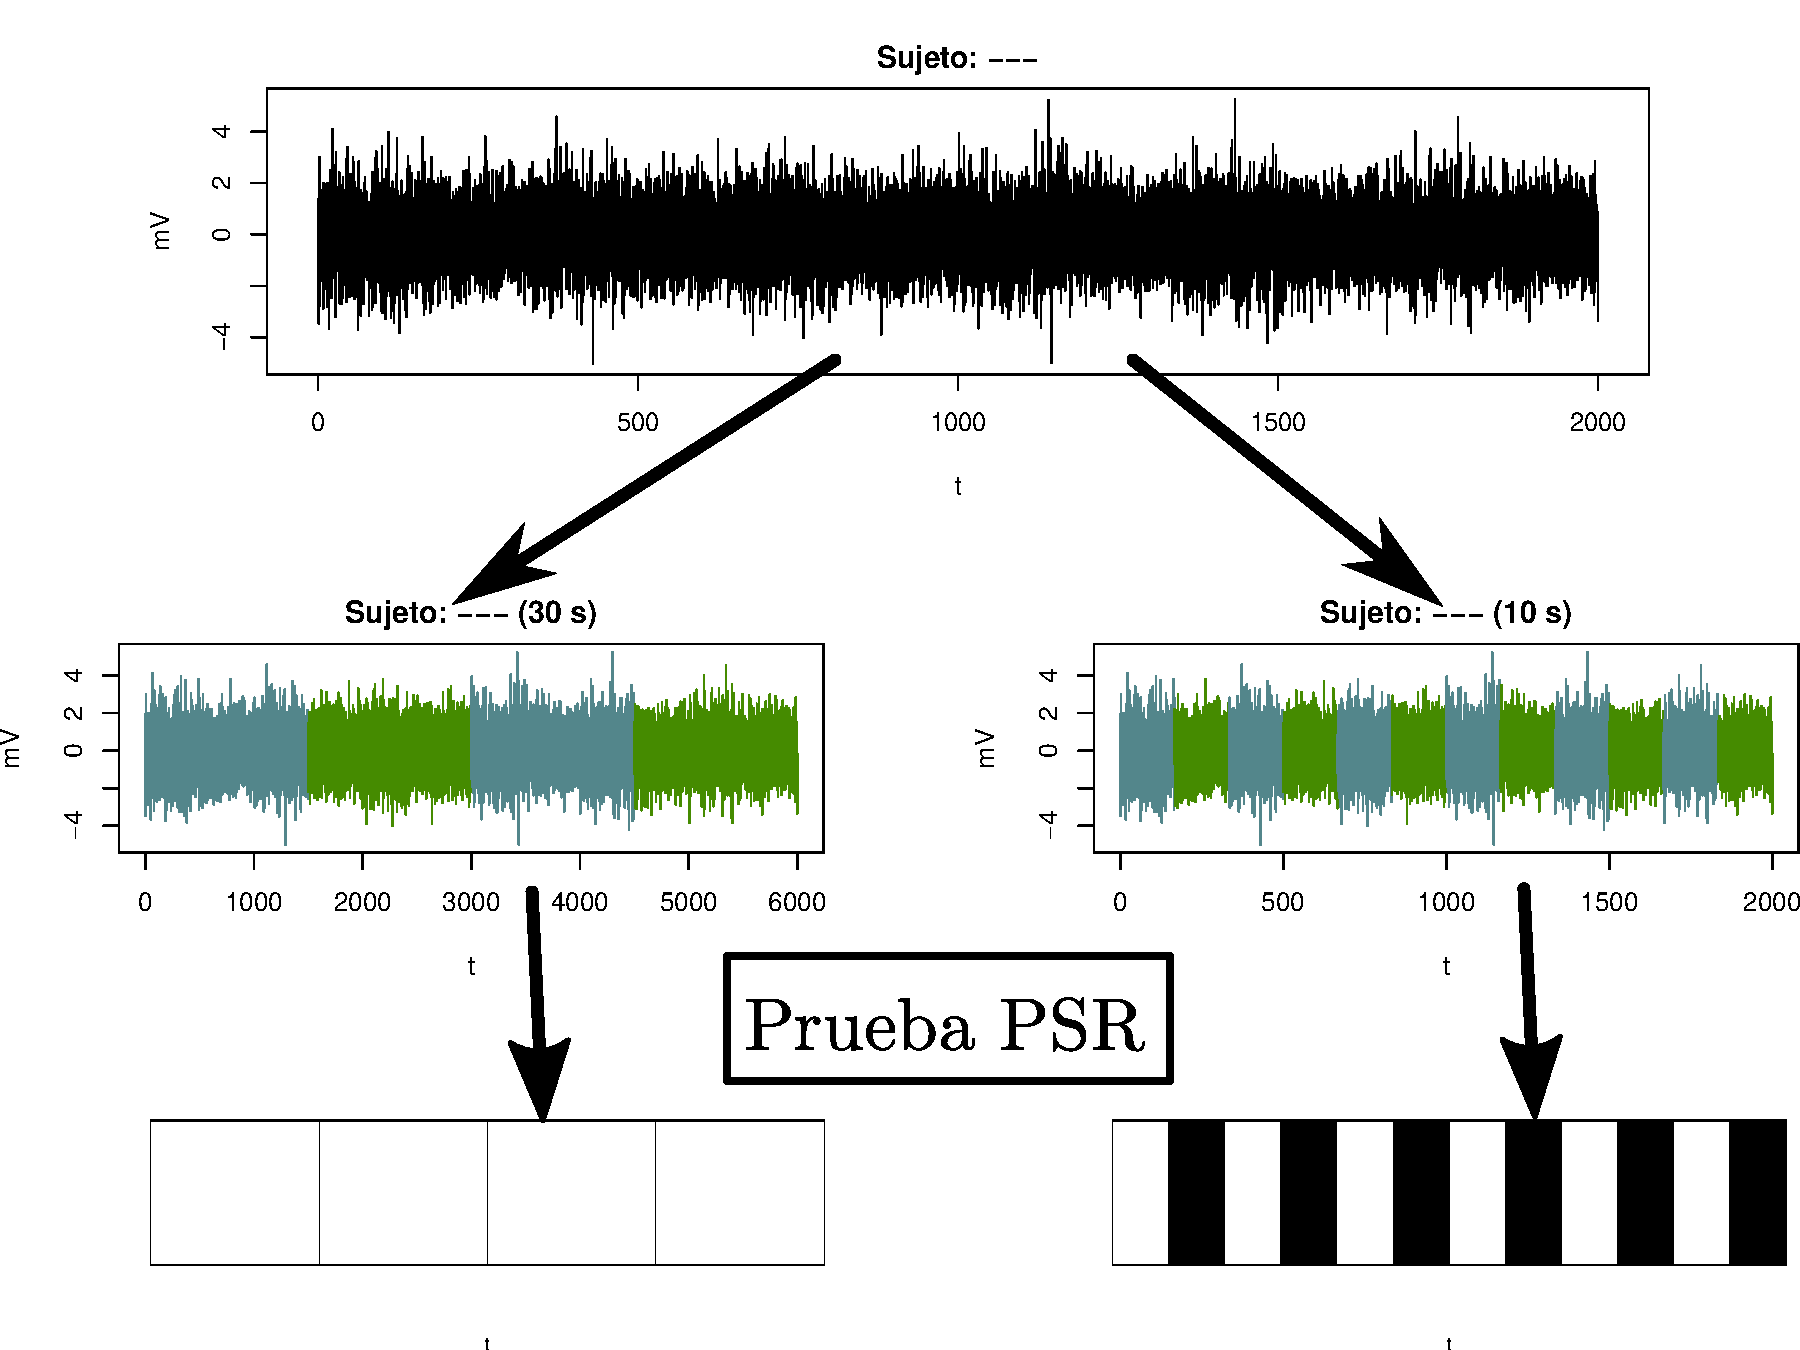
\includegraphics[width=0.9\linewidth]{./img_diagramas/epocas_diferentes.pdf}
%\caption{En el PSG}
\end{figure}
\end{frame}

\begin{frame}\frametitle{Sobre el tama\~no de la \'epoca}
\begin{figure}
\centering
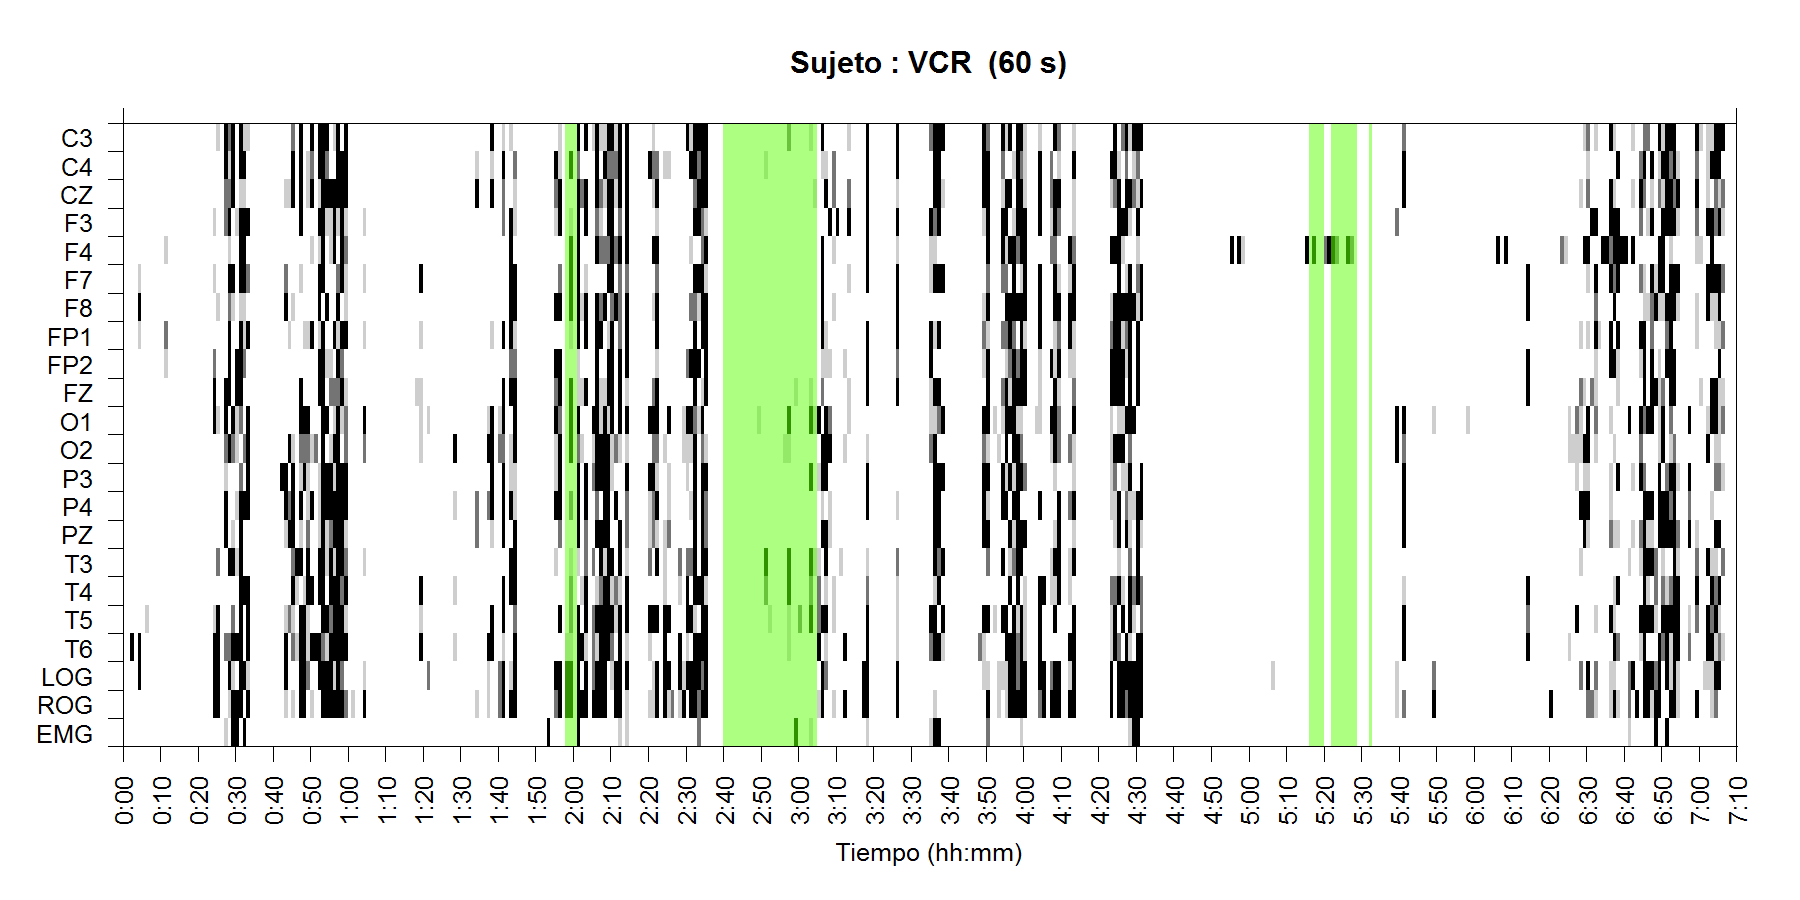
\includegraphics[width=0.9\linewidth]
{./img_ejemplos/VCNNS1_est_60.png} 
\end{figure}
\end{frame}

\begin{frame}\frametitle{Sobre el tama\~no de la \'epoca}
\begin{figure}
\centering
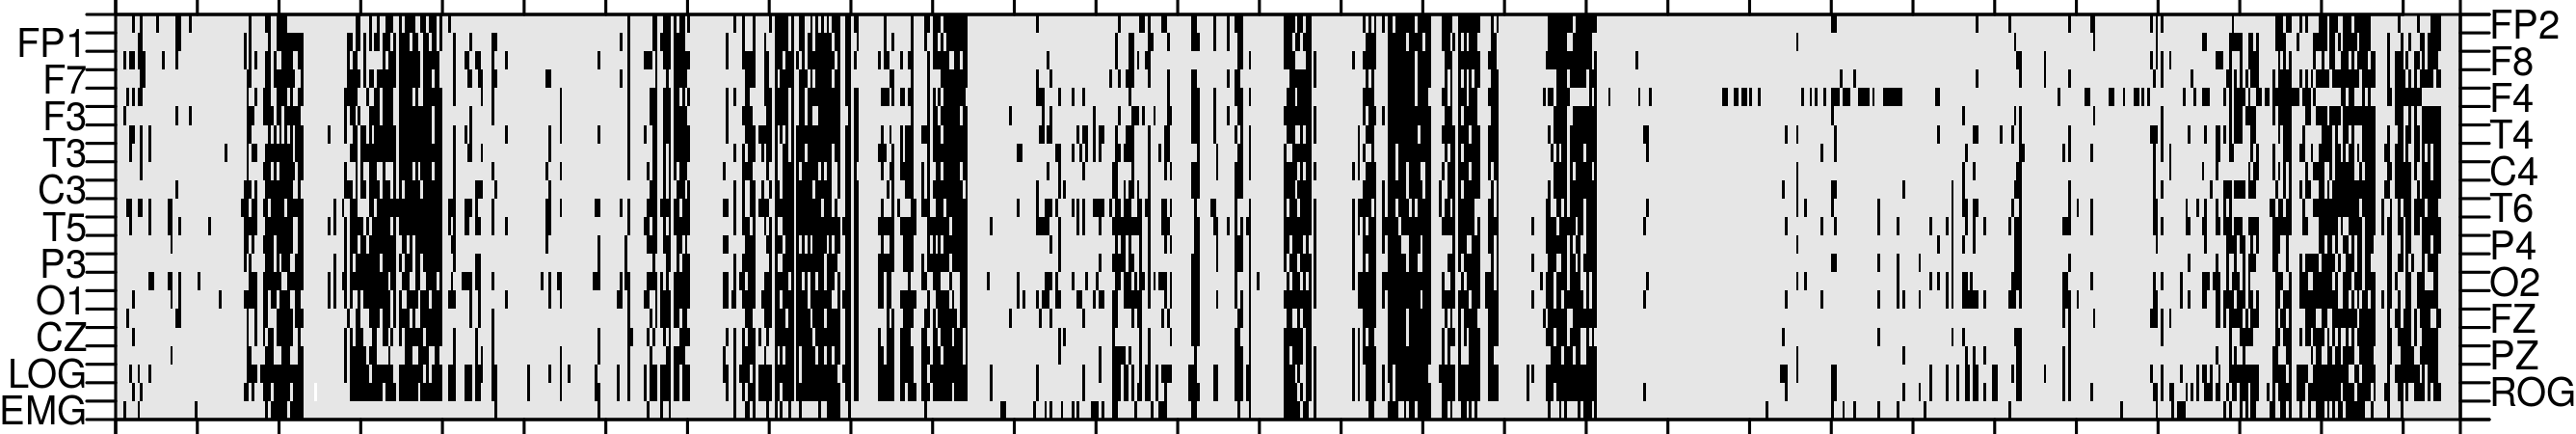
\includegraphics[width=0.9\linewidth]
{./img_ejemplos/VCNNS1_est_30.png} 
\end{figure}
\end{frame}

\begin{frame}\frametitle{Sobre el tama\~no de la \'epoca}
\begin{figure}
\centering
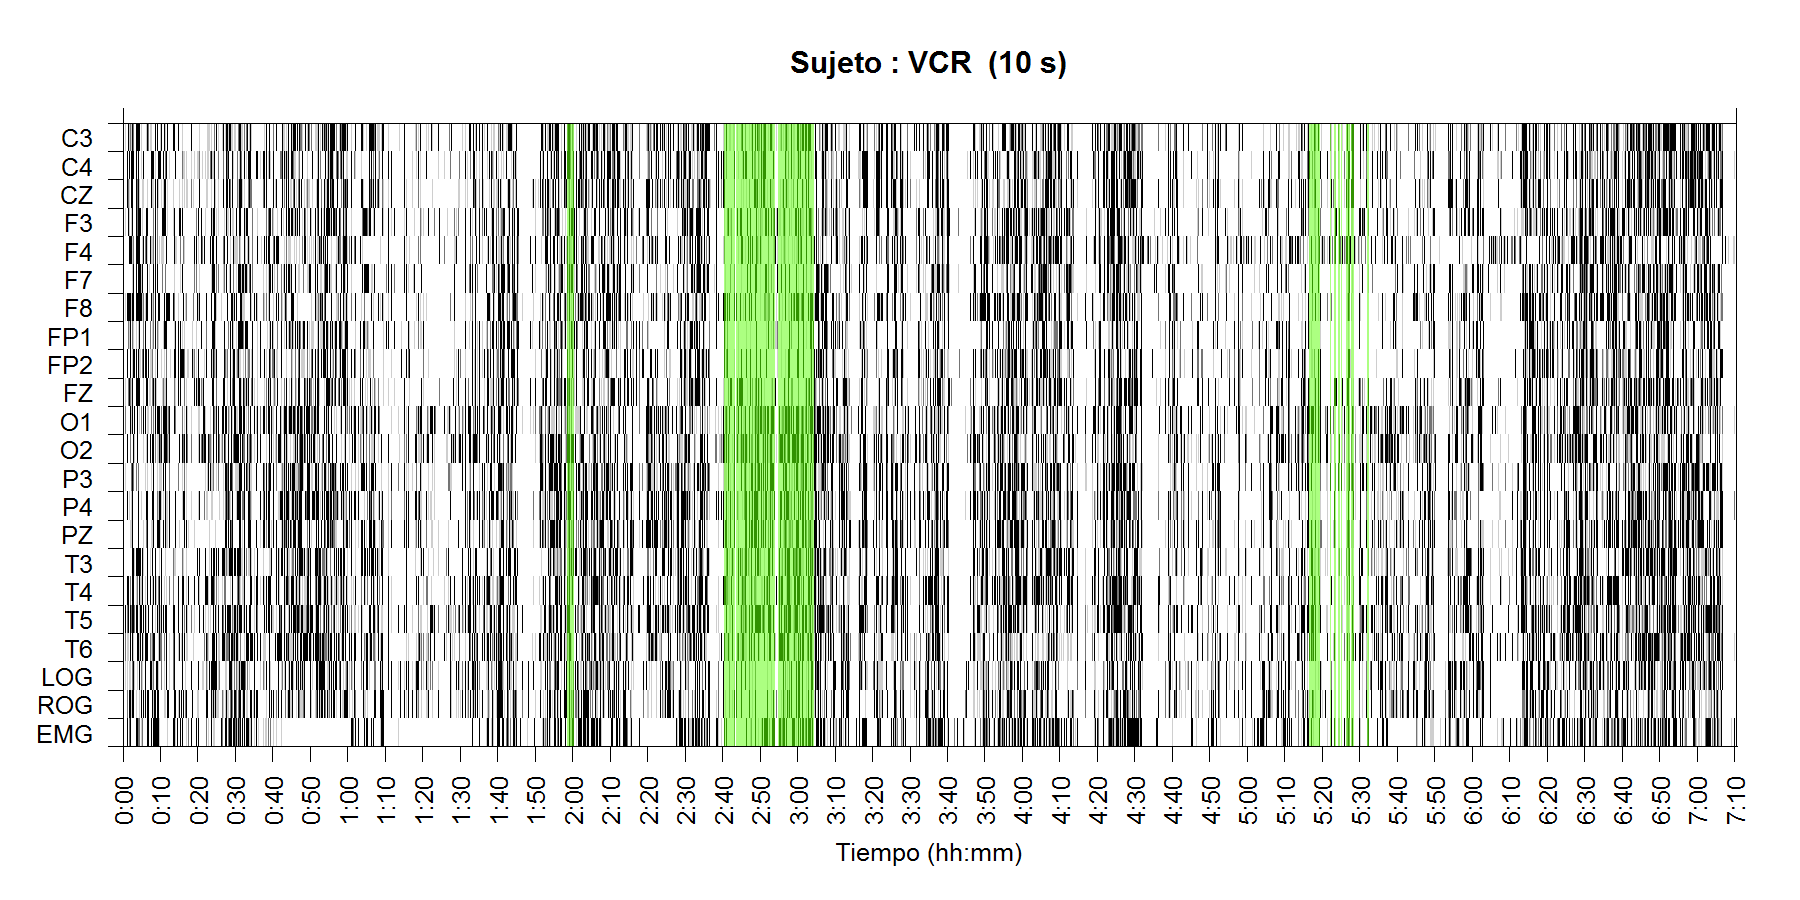
\includegraphics[width=0.9\linewidth]
{./img_ejemplos/VCNNS1_est_10.png} 
\end{figure}
\end{frame}

%%%%%%%%%%%%%%%%%%%%%%%%%%%%%%%%%%%%%%%%%%%%%%%%%

\begin{frame}\frametitle{Sobre el tama\~no de la \'epoca}
{\small Estacionariedad local\footcite{Cohen77}}
\begin{figure}
\centering
\begin{tabular}{c}
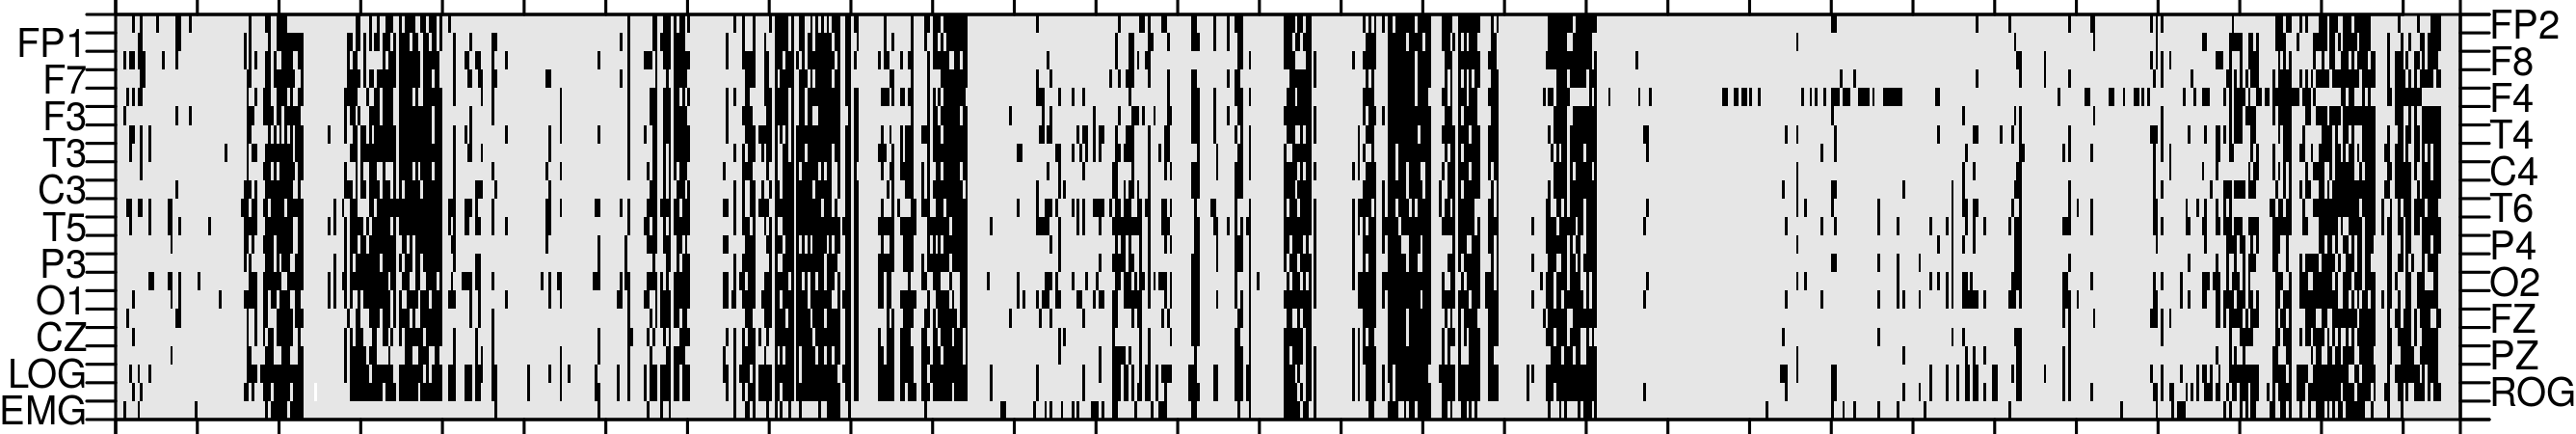
\includegraphics[width=0.4\linewidth]
{./img_ejemplos/VCNNS1_est_30.png} \\
\begin{tabular}{cc}
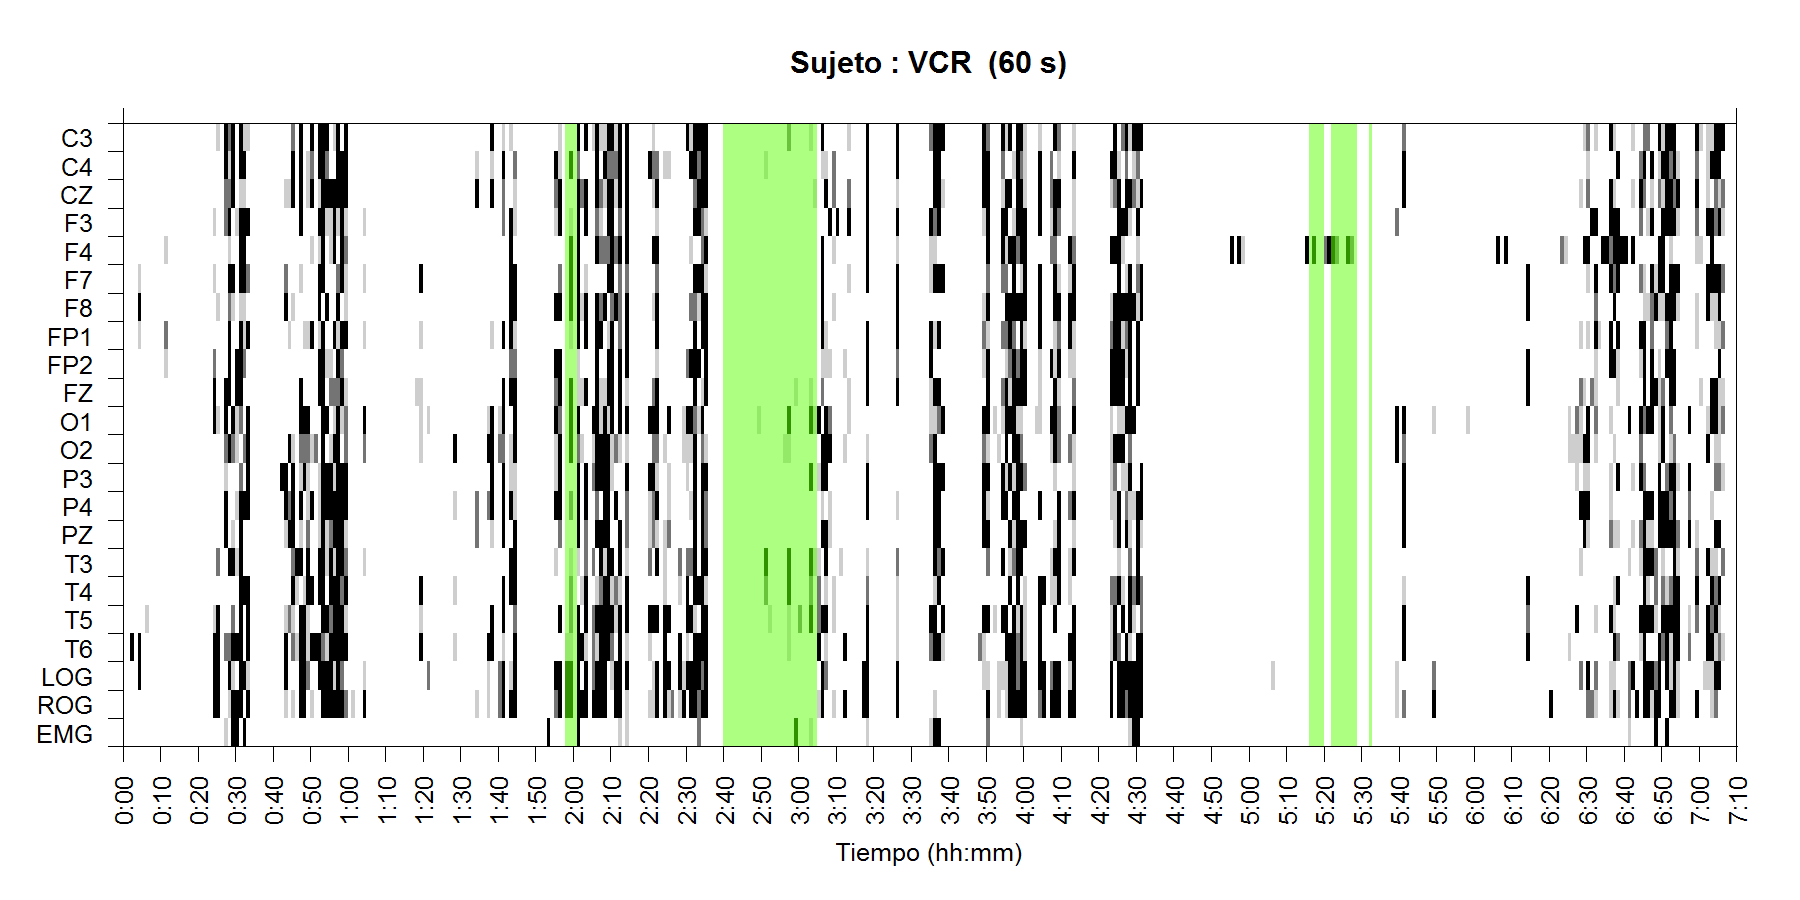
\includegraphics[width=0.4\linewidth]
{./img_ejemplos/VCNNS1_est_60.png} 
&
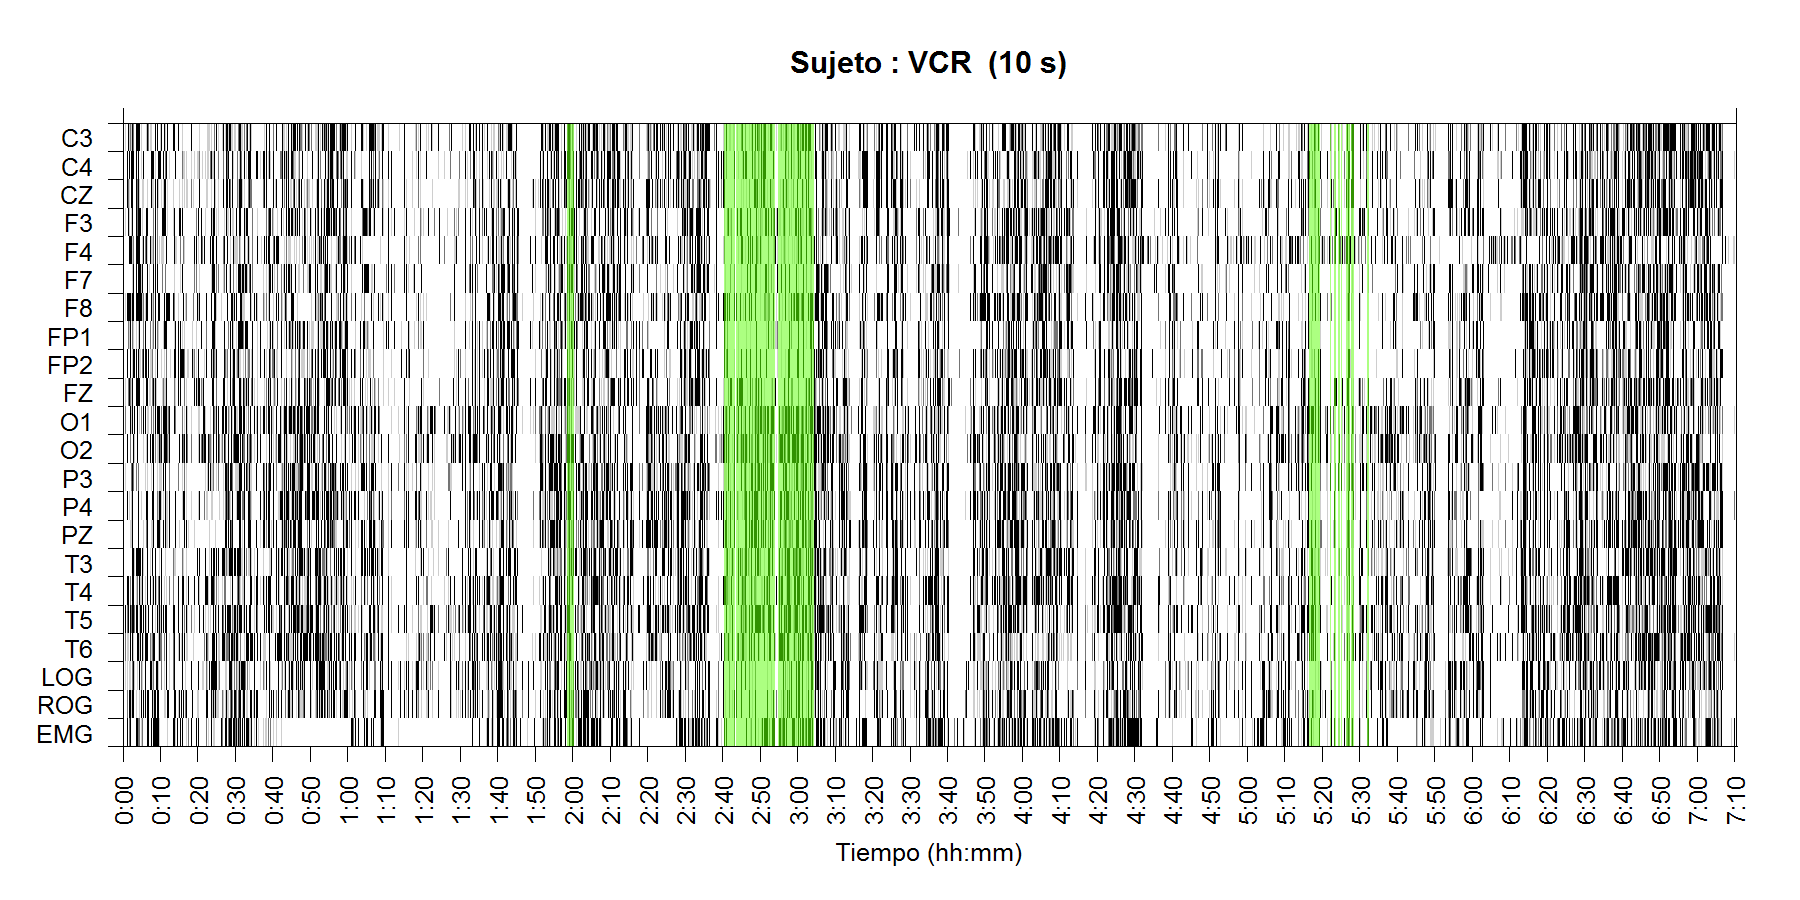
\includegraphics[width=0.4\linewidth]
{./img_ejemplos/VCNNS1_est_10.png} 
\end{tabular}
\end{tabular}
\end{figure}
\end{frame}

%%%%%%%%%%%%%%%%%%%%%%%%%%%%%%%%%%%%%%%%%%%%%%%%%

%\begin{frame}\frametitle{Gracias por su atenci\'on}
%\begin{figure}
%\centering
%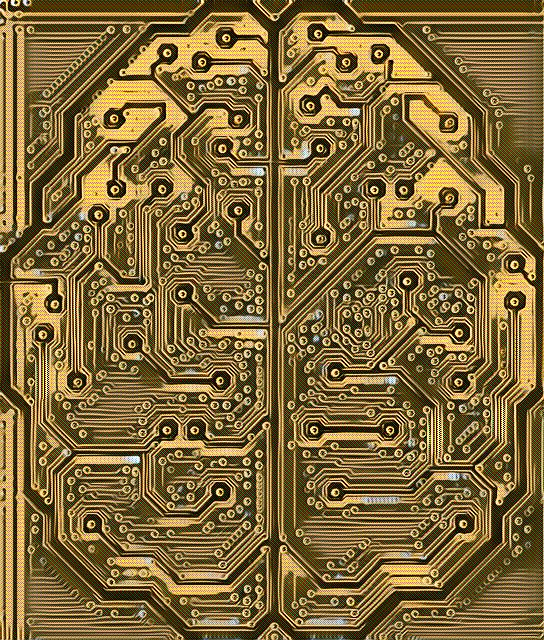
\includegraphics[width=0.4\linewidth]{./img_adornos/cerebot.jpg}\\
%\vspace*{1em}
%\textit{El cerebro es, quiz\'a, el \'unico \'organo capaz de estudiarse a s\'i mismo.}
%\end{figure}
%\end{frame}

%%%%%%%%%%%%%%%%%%%%%%%%%%%%%%%%%%%%%%%%%%%%%%%%%

\end{document}

%%%%%%%%%%%%%%%%%%%%%%%%%%%%%%%%%%%%%%%%%%%%%%%%%%%%%%%%%%%%%%%%%%%%%%%%%%%%%%%%%%%%%%%%%%%%%%%%%%%